\section{Basics of 3D-PTV and real-time 3D-PTV}
\topicFramePrimary{3D-PTV: essential factors and prerequisites}


% \begin{frame}
%     \frametitle{Feasibility and Difficulty}
%     \begin{itemize}
%     \item Discuss the technical feasibility of real-time 3D-PTV and the challenges that must be overcome to achieve it.
%     \item Highlight some of the key research areas that need to be addressed to make real-time 3D-PTV more feasible and efficient.
%     \item Provide examples of some of the tools and resources available to help researchers in this area.
%     \end{itemize}
% \end{frame}
    

\begin{frame}[label=ptv-1]{3D-PTV overview}
    \begin{multicols}{2}
    \begin{card}[What is 3D-PTV]
    3D-PTV is a technique that allows tracking of particles in three-dimensional space for improved fluid dynamics understanding, using the Lagrangian framework
    \end{card}
    \begin{card}[TL;DR]
    Multiple 2D projections of the particles are obtained and overlapped to create 3D reconstruction. Software than tracks the particles' positions through sequential images over time. 
    \end{card}
    \end{multicols}
\end{frame}


%
\begin{frame}[label=ptv-2]{Shr\"{o}der and Schanz, Annu. Rev. Fluid Mech. 2023}
    \cardImg{shroder.jpeg}{\textwidth}
\end{frame}

\begin{frame}[label=ptv-3]{This sculpture helped people to feel like a Lagrangian particle}
    \centering\cardImg{art}{0.8\textwidth}
    \vspace{-.3cm}
    \begin{cardTiny}
    ``Marianthe'' invited people inside turbulent forms to experience them as
    if they were a particle borne along in the flow. Athena
    Tacha (1985), \href{http://nautil.us/issue/15/turbulence/the-scientific-problem-that-must-be-experienced}{``Nautilus'' by Philip Ball}
    \end{cardTiny}                                                          
\end{frame}
%

\begin{frame}[label=ptv-4]{Let's get a quick intro to 3D-PTV}
    \cardImg{ptv-scheme}{1.0\textwidth}
\end{frame}
% % 
% % %
% \begin{frame}[label=ptv-2]{Basic steps}
% \begin{columns}[t]
% 	\begin{column}{0.4\textwidth}
% 		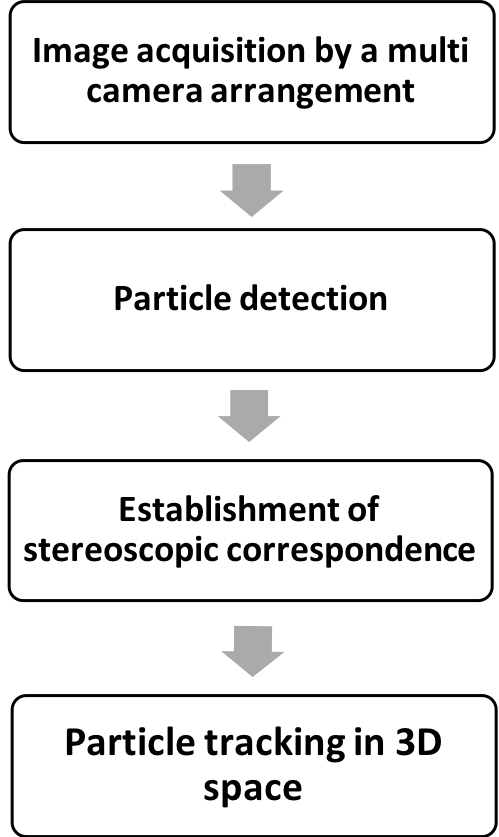
\includegraphics[height=.8\textheight]{ptv_blocks}
% 	\end{column}
% 	\begin{column}{0.3\textwidth}
% 		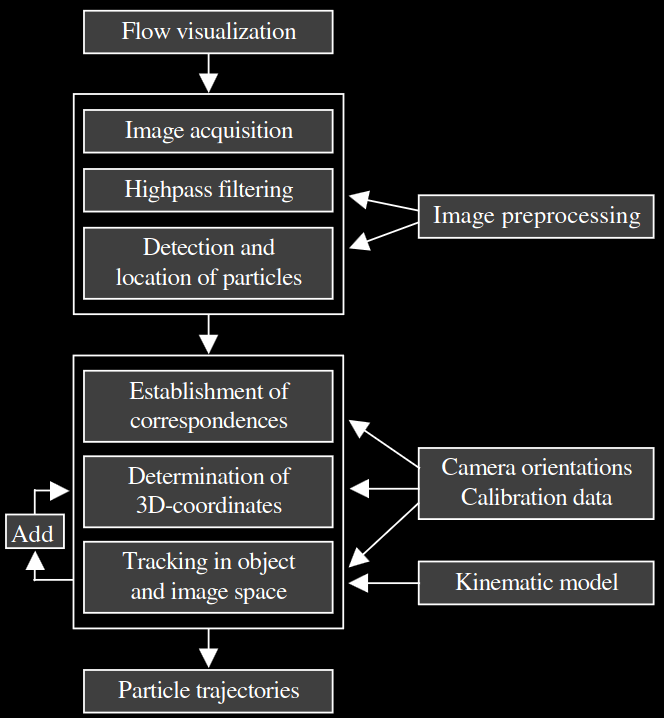
\includegraphics[height=.8\textheight]{ptv_steps}
% 	\end{column}
% \end{columns}
% \end{frame}


\begin{frame}[label=ptv-5]{Basic steps of 3D-PTV}
    \centering\cardImg[height=.8\textheight]{ptv_steps}{\textwidth}
\end{frame}

% %%
% \begin{frame}[label=ptv-22]{Basic steps}
% \begin{multicols*}{2}
% 		\cardImg[height]{ptv_blocks}{.49\textwidth}
% 		\cardImg[height]{ptv_steps}{.49\textwidth}
% \end{multicols*}
% \end{frame}

\begin{frame}[label=ptv-6]{Epipolar geometry}
    \centering\cardImg{epipolar1}{1\textwidth}
\end{frame}

\begin{frame}[label=ptv-7]{Multi-view epipolar geometry}
    \centering\cardImg{epipolar}{\textwidth}
\end{frame}

\begin{frame}[label=ptv-8]{That's how it looks in software}
    \centering\cardImg{stereo_matching}{\textwidth}
\end{frame}

\begin{frame}[label=ptv-9]{It strongly depends on 3D calibration}
    \centering\cardImg{calibration1}{\textwidth}
\end{frame}


\begin{frame}[label=ptv-9]{We prefer multi-media non-linear calibration}
    \centering\cardImg[height=.8\textheight]{multimedia}{\textwidth}
\end{frame}

\begin{frame}[label=ptv-10]{Four frames sliding tracking}
    \centering\cardImg{tracking}{1\textwidth}
\end{frame}

\begin{frame}[label=ptv-11]{Tracking in 2D space}
    \centering\cardImg[height=.8\textheight]{tracking_in_image_space_projection}{1\textwidth}
\end{frame}


\begin{frame}[label=ptv-12]{Tracking in 2D space}
	\centering\cardImg[height=.8\textheight]{tracking_in_image_space}{1\textwidth}
\end{frame}


\begin{frame}[label=ptv-13]{Tracking in 3D space }
	\centering\cardImg[height=.8\textheight]{tracking_in_3d_space}{1\textwidth}
\end{frame}


\begin{frame}[label=ptv-14]{Tracking in both 2D and 3D}
	\centering\cardImg[height=.8\textheight]{image_space_tracking}{1\textwidth}
\end{frame}

			

\begin{frame}[label=ptv-15]{The results are Lagrangian trajectories, $X(a,t)$}
    %\begin{multicols}{2}
    \centering
    \cardImg{lagrangian_trajectory}{.9\textwidth}
    % \cardImg{particle_trajectories}{.39\textwidth}
    % \end{multicols}
\end{frame}


\begin{frame}[label=ptv-16]{Two-frame PTV is somewhere between Eulerian and Lagrangian}
    \centering\cardImg{eulerian_vs_lagrangian}{\textwidth}
\end{frame}

% \begin{frame}[label=ptv-8]
% \frametitle{Time-resolved is a tautology, real-time is real :) }
% \begin{enumerate}
% \item Time-resolved PTV is a tautology - to track objects we have to resolve their position in time :) 
% \item Real-time is not at the velocity of the particle, but during the experiment: we get trajectories on the screen when the flow is moving (not the same flow)
% \end{enumerate}
% \end{frame}

